\documentclass[addpoints, 12pt] {exam}
\usepackage{graphicx}
\usepackage{amsmath}
\bracketedpoints
\pagestyle{headandfoot}
\runningheadrule
\firstpageheader{Math 112}{Written Homework 2}{Due January 26th 2024}
\runningheader{Math 112}{ Page\; \thepage\; of\; \numpages}{Written Homework 2}
\firstpagefooter{}{}{}
\runningfooter{}{}{}
\setlength\answerskip{2ex}
\setlength\answerlinelength{1.5in}
\begin{document}

\begin{center}
\fbox{\fbox{\parbox{5.5in}{\centering
Directions:\\Please only put your final, well written solutions, in the space provided.\\ Give exact answers (simplified radicals or fractions).\\If you use additional paper clearly label the question and upload pages after the question page.\\Use complete sentences and explain your reason as much as possible.\\There are \numquestions\,  questions and \numpoints\, points total
}}}\end{center}
\vspace{0.1in}
\makebox[\textwidth]{Name:\enspace\hrulefill}
%\qformat{Question \thequestion \dotfill \thepoints}%

\begin{questions}
\question \textbf{Note:} I \emph{know} you can graph this entirely on Desmos and just copy it. Please do not do this.  \emph{After} you complete the sketch, it is fine to double check yourself, but the goal with this question is for you to build up to the graph using your own reasoning and calculations!.

Many people enjoy coffee as one of their first drinks in the morning (many also enjoy tea too!). Suppose that the following models the amount of caffeine (in mg) in a person's body \(t\) hours after they consume it (we will ignore the time it takes to drink the coffee): \[A(t) = 150\left(\frac{2}{5}\right)^{t/6}\]
\begin{parts}
\part[1] For a single cup of coffee, and based on your own experiences, provide a reasonable domain for this function. You will use this domain when sketching the graph later, so feel free to change this if it doesn't work out when graphing in part (c).\answerline
\part[2] Given the domain you picked above, create a \textbf{table of input/output values} that cover the whole domain you chose. For example, if you put that the domain is \([0,12]\), then picking the following input values \(0, 0.5, 1, 1.5, 2, 2.5, ... 11.5, 12\) would give you good coverage of the domain. Pick at least 10 input values.
\newpage
\part[3] Sketch a graph of the function based on your domain and table of values. You may use a separate piece of paper.\vspace{4in}
\part[1] Based on \emph{your} sketch, where is this function increasing?
\answerline
\part[1] Based on \emph{your} sketch, where is this function decreasing?
\answerline
\part[1] Based on \emph{your} sketch, after how many hours is the concentration of caffeine in your blood steam at its maximum? \answerline
\part[1] Based on \emph{your} sketch, if the caffeine is only effective when there are at least \(50\)mg in the your bloodstream, how long is a single cup effective? Round your answer to the nearest hour. \answerline 
\end{parts}\newpage
\question The graph below shows a function which measures a runner's distance from the recreation center as they go for their morning run. They started their run at 5:00am. Use this graph to answer the questions below.\newline 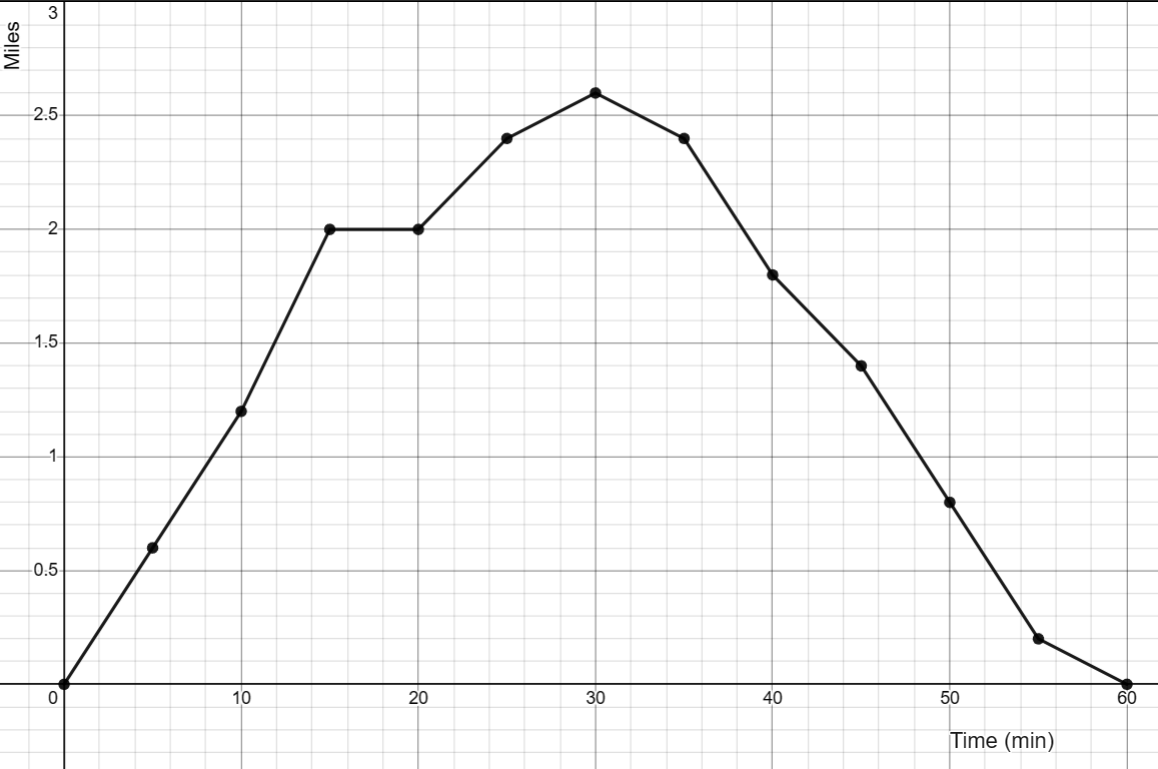
\includegraphics[scale=0.45]{timevdistance}\newline
\begin{parts}
\part[1] What does the vertical intercept mean, in practical terms? Provide a written explanation.\vspace{1.25in}
\part[1] What does the larger horizontal intercept mean, in practical terms? Provide a written explanation.
\vspace{1.25in}
\part[1] What is the domain of this function?\answerline
\part[1] What is the range of this function?\answerline
\part[2] On which intervals is this function \textbf{increasing}?\answerline
\part[2] On which intervals is this function \textbf{decreasing}?\answerline
\part[1] On which intervals is this function \textbf{constant}?\answerline
\part[1] Describe the last 5 minutes of their run compared to the rest of their run.
\end{parts}

\newpage
\question A patient has been prescribed a course of antibiotics to combat a bacterial infection. The drug is administered in doses and is absorbed into the patient's bloodstream. Human bodies will naturally filter the antibiotics out over time. The total amount of antibiotics, in mg, in the patient's bloodstream \(t\) hours after the dose is given can be modeled with the function \[A(t) = 500te^{-0.5t}\]
\begin{parts}
\part[1] For a single dose, and using your own experience with medication, provide a reasonable guess for the domain of this function. You will use this guess when sketching the graph later, so feel free to change this if it doesn't work out when graphing in part (c).\answerline
\part[2] Given the domain you picked above, create a \textbf{table of input/output values} that cover the whole domain you chose. For example, if you put that the domain is \([0,12]\), then picking the following input values \(0, 0.5, 1, 1.5, 2, 2.5, ... 11.5, 12\) would give you good coverage of the domain. Pick at least 10 input values.
\newpage
\part[3] Sketch a graph of the function based on your domain and table of values. You may use a separate piece of paper. \vspace{4in}
\part[1] Based on \emph{your} sketch, where is this function increasing?
\answerline
\part[1] Based on \emph{your} sketch, where is this function decreasing?
\answerline
\part[1] Based on \emph{your} sketch, after how many hours is the concentration of antibiotics in your blood steam at its maximum? \answerline
\part[1] Based on \emph{your} sketch, if the antibiotics are only effective when there are at least \(100\)mg in the patient's bloodstream, how long is a single dose effective? Round your answer to the nearest hour. \answerline 
\end{parts}
\newpage
\question Suppose you are considering converting your gas powered water heater to a solar water heater. The gas heater is already installed in your home and costs, on average, $\$450$ per year. After consulting different companies, you find one who offers to install the solar water heater for $\$5,000$ and will cost, on average, $\$40$ in electricity to run the pumps each year.
\begin{parts}
\part[2] Write the equation for the cost, $C_g$, for the gas powered water heater. Use $t$ for your input variable. \answerline
\part [2] Write the equation for the cost, $C_s$, for the solar powered water heater. Use $t$ for your input variable. \answerline
\part[6] After installation, how many years will you need to be on solar power to balance with the cost of just sticking with gas? Show your work.\vspace{3in}\answerline
\end{parts}


\end{questions}


\end{document}